\PassOptionsToPackage{unicode}{hyperref}
\PassOptionsToPackage{aux}{rerunfilecheck}

\documentclass[aspectratio=1610]{beamer}

\usepackage{polyglossia}
\setmainlanguage{german}

\usepackage{amsmath}
\usepackage{amssymb}
\usepackage{mathtools}

\usefonttheme{professionalfonts}
\usepackage{fontspec}
\usepackage[
math-style=ISO,
bold-style=ISO,
nabla=upright,
partial=upright,
sans-style=italic,
]{unicode-math}
\setmathfont{Latin Modern Math}

\usepackage[
  math-micro=µ,
  locale=DE,
]{siunitx}

\usetheme{Frankfurt}
\usecolortheme{seagull}
\setbeamertemplate{navigation symbols}{}



% ImDokument:
% \author{...}
% \institute{...}
% \date{...}
% \title{...}

% \maketitle im ersten Frame
%\tableofcontents für ein Inhaltsverzeichnis


\usetheme{Warsaw}

%%% Fusszeile und deren Farbedefinitionen aus dem outertheme infolines
\setbeamercolor*{author in head/foot}{parent=palette tertiary}
\setbeamercolor*{title in head/foot}{parent=palette secondary}
\setbeamercolor*{date in head/foot}{parent=palette primary}
\makeatletter
\setbeamertemplate{footline}
{
  \leavevmode

  \hbox{

  \begin{beamercolorbox}[wd=.33\paperwidth,ht=2.25ex,dp=1ex,center]{author in head/foot}
    \usebeamerfont{author in head/foot}\insertshortauthor\expandafter\beamer@ifempty\expandafter{\beamer@shortinstitute}{}{~~(\insertshortinstitute)}
  \end{beamercolorbox}

  \begin{beamercolorbox}[wd=.33\paperwidth,ht=2.25ex,dp=1ex,center]{title in head/foot}
    \usebeamerfont{title in head/foot}\insertshorttitle
  \end{beamercolorbox}

  \begin{beamercolorbox}[wd=.33\paperwidth,ht=2.25ex,dp=1ex,right]{date in head/foot}
    \usebeamerfont{date in head/foot}\insertshortdate{}\hspace*{2em}
    \insertframenumber{} / \inserttotalframenumber\hspace*{2ex}
  \end{beamercolorbox}}

  \vskip0pt
}
\makeatother

%\usetheme{Singapore}
%\setbeamertemplate{sections/subsections in toc}[sections numbered]
%\setbeamertemplate{subsection in toc}[subsections numbered]

\author{Sebastian Pape \and Jonah Nitschke}
\institute{TU Dortmund}
\date{\today}
\title{Zusatzversuch: Die Wirbelstrombremse}
\subtitle{Anfängerpraktikum Physik III}


\begin{document}

  \begin{frame}[plain]
    \titlepage
  \end{frame}

  \section{Einleitung in den Versuch und Idee}

  \begin{frame}

      \begin{columns}[onlytextwidth]
        \begin{column}{0.45\textwidth}
          \begin{figure}
            \centering
              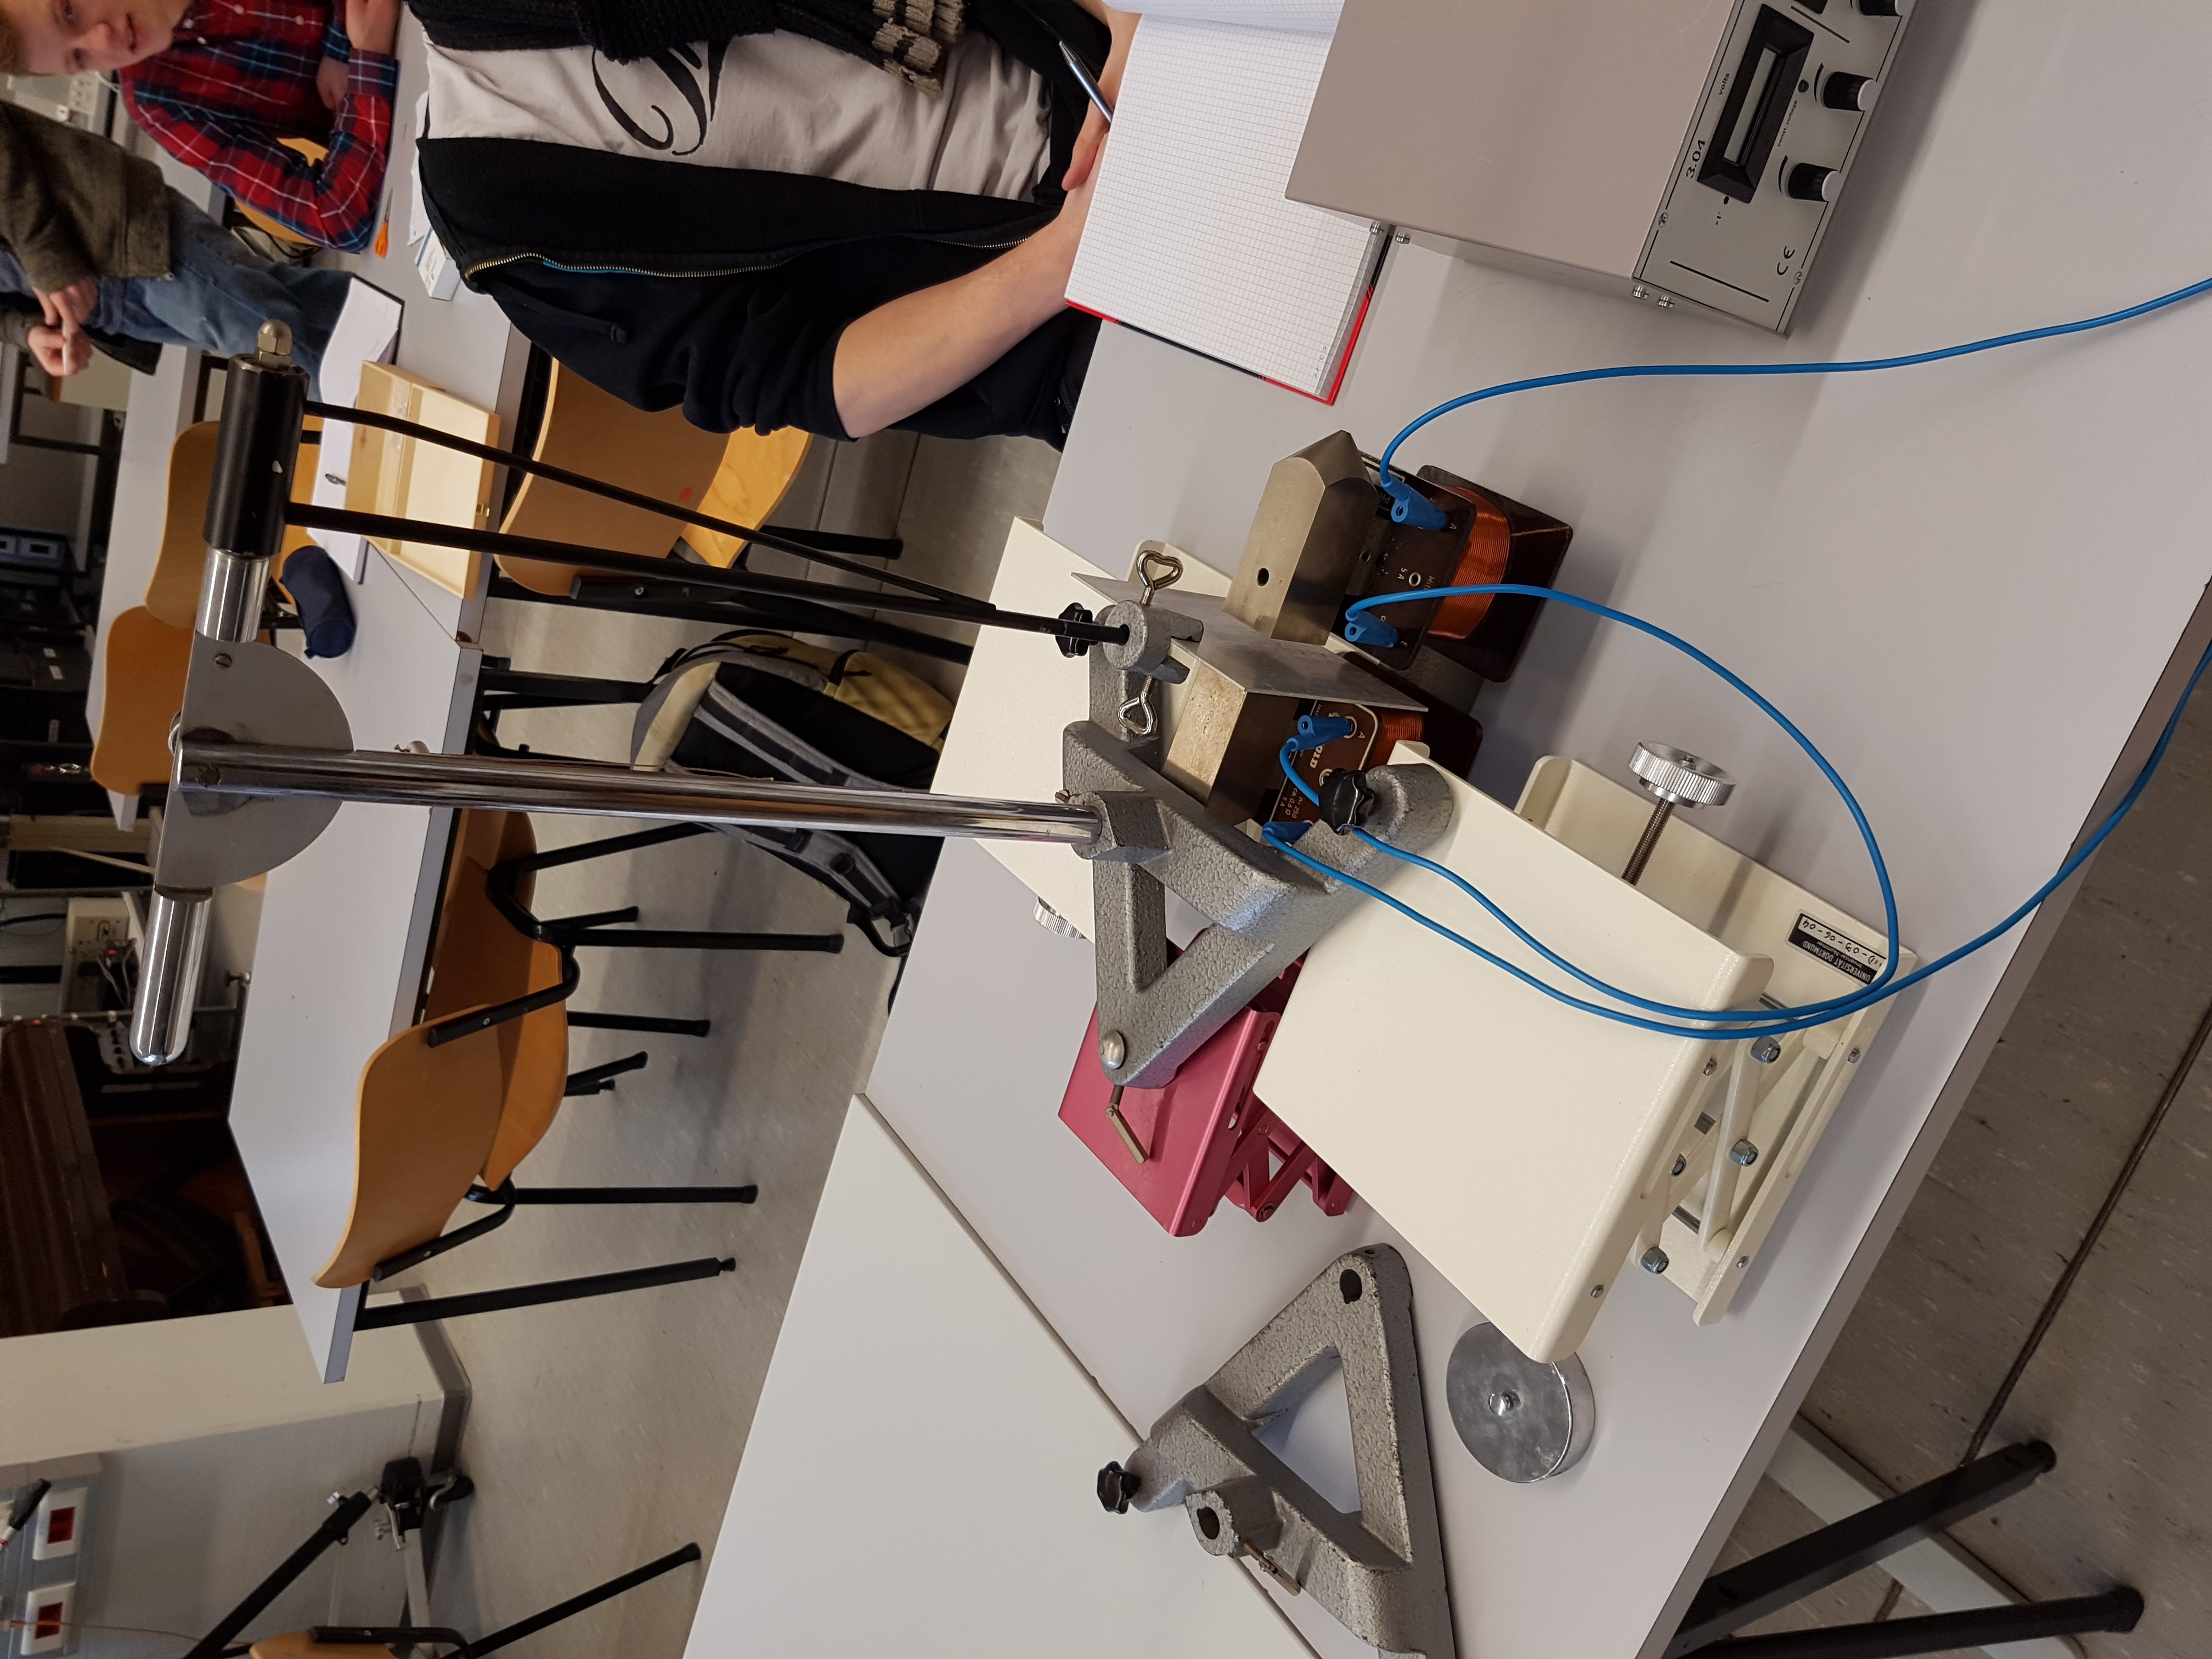
\includegraphics[height=5cm, angle = -90]{20170306_101228.jpg}
          \end{figure}
        \end{column}
        \begin{column}{0.45\textwidth}
          \begin{figure}
            \centering
              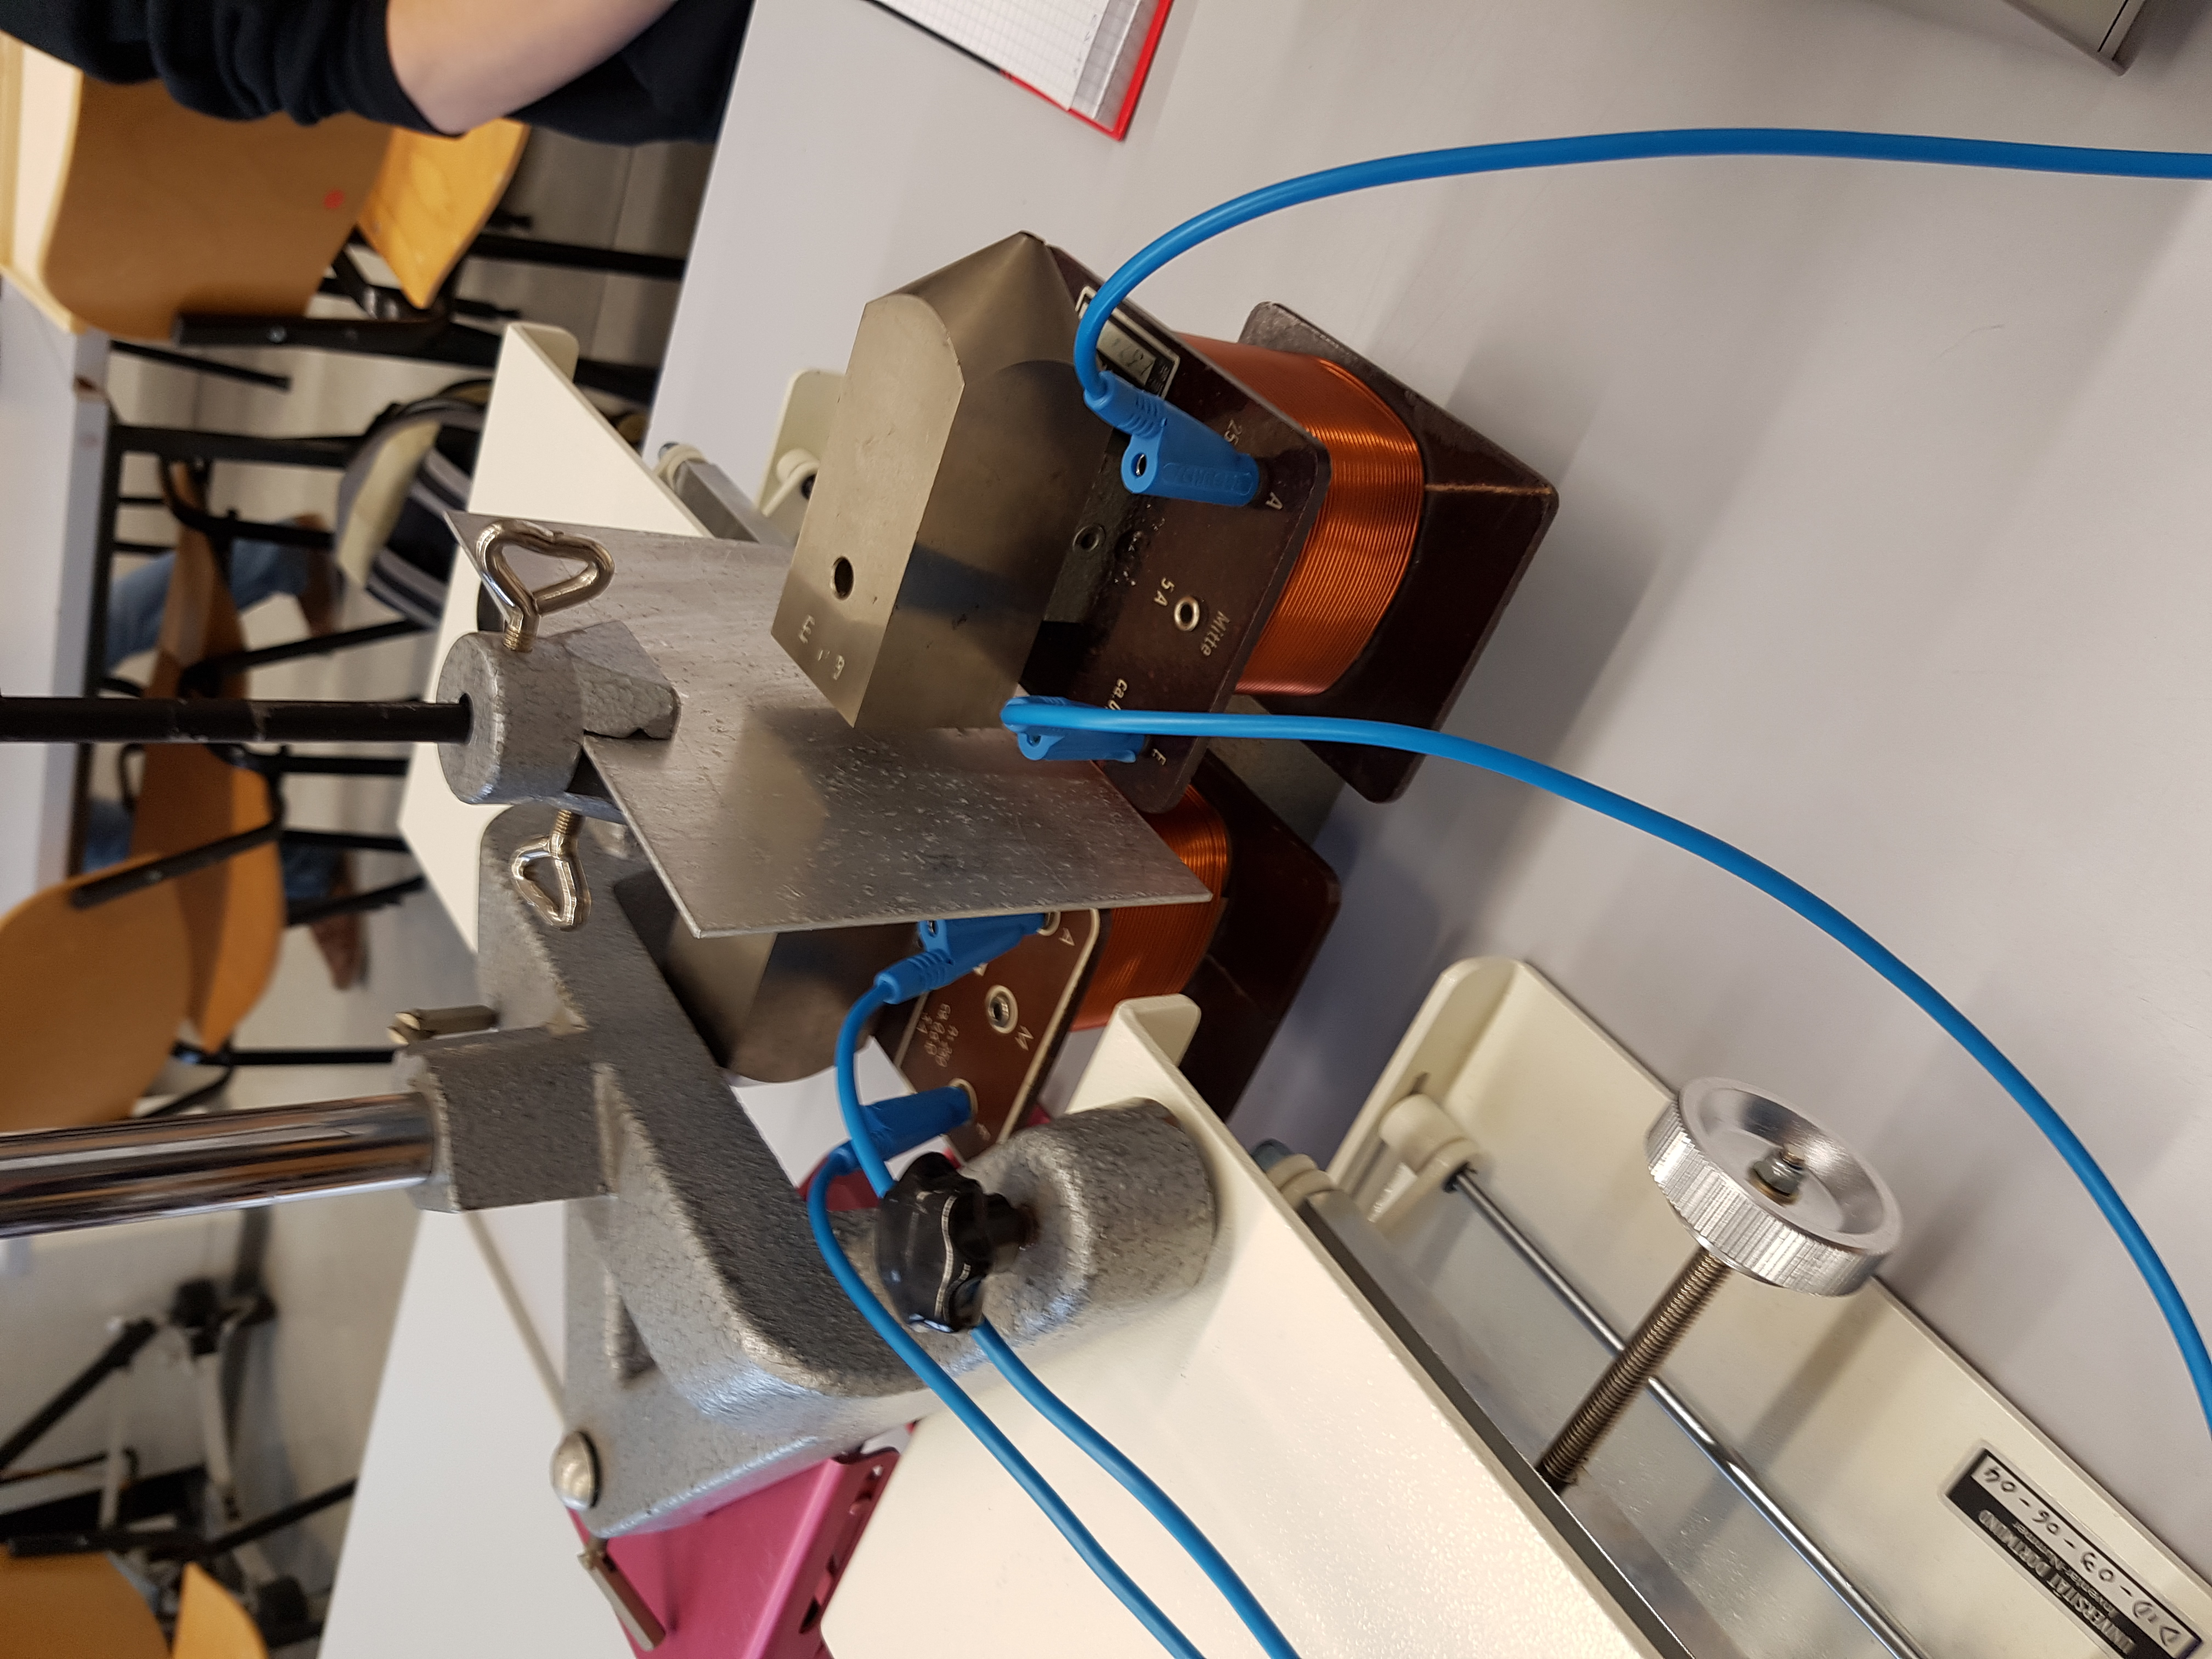
\includegraphics[height=5cm, angle = -90]{20170306_101230.jpg}
          \end{figure}
        \end{column}
      \end{columns}

  \end{frame}

  \section{Aufbau}

  \begin{frame}
    Dieser Text ist nur um das Thema zu testen!
  \end{frame}
\end{document}
